The SM is chiral, meaning that left- and right-handed particles transform differently under the weak interaction, as we learned in Section \ref{sec:SM}. This prevents us from writing fermionic mass terms in the Lagrangian, resulting in the need to introduce a scalar to spontaneously break the gauge symmetry to generate massive fermions (and gauge bosons). Therefore, to better understand the high-energy behaviour of SM extensions, it is necessary to apply the CAF framework from Chapter \ref{chap:CAF} to chiral gauge-Yukawa theories with scalars. To follow a top-down approach, the goal is to identify minimal CAF models, that can serve as viable high-energy theories.

In this chapter we will introduce two chiral models. The generalised Georgi--Glashow (GG) \cite{Georgi:1974yf} and the Bars--Yankielowicz (BY) \cite{Bars:1981se} model. In Section \ref{sec:noscalar} we consider both models separately without scalars. Then in Section \ref{sec:fundscalar}, we introduce a fundamental scalar. Finally we introduce an adjoint scalar in Section \ref{sec:adj}. These two representations of scalars follow from the general need of a scalar to break the gauge group down to the SM gauge structure and one to play the role of the Higgs, as reviewed in Section \ref{sec:SU5}. 


\section{Introduction of the Chiral Models} \label{sec:noscalar}
The models we will consider consist both of vector-like fermions and chiral fermions transforming under the same non-Abelian gauge group $\SU(N)$. We thus have: the anti-fundamental fermion $\tilde\psi$, the fundamental fermion $\psi$, and the two-index fermion $\Lambda$. The two-index fermion is chiral and therefore lacks a corresponding anti-fermionic field to generate a bare mass term. To extrapolate the models' behaviour at high energies, we need to compute beta functions, which are derived directly from the Lagrangian. 

The fundamental first step is to write down a Lagrangian that respect both the gauge symmetry and the global symmetries. Then, we generalise the model by allowing for $p$ fundamental and $q$ anti-fundamental fermions. The number of flavours will directly affect the gauge anomaly calculation. To ensure a viable quantum theory, the gauge symmetry must be anomaly-free, a condition that is not automatically satisfied for Weyl fermions as it is for Dirac fermions \cite{Peskin:1995ev}. The anomaly arises from triangle diagrams \cite{tong}, which impose the following conditions (see Appendix \ref{app:Lie})
\begin{align}
    \tr(T^a_R\{T^b_R,T^c_R\})&=A(R)d^{abc}\,,\\\sum \mu_i A(R_i)&\overset{!}{=}0\,,\label{eq:gaugeanomaly}
\end{align}
where $\mu_i$ is the multiplicity of each representations $R_i$ and $A(r)$ is the anomaly coefficient. The condition of the anomaly cancellation effectively introduces a relation between $p$, $q$, and the number of colours $N$.

Besides the two global flavour symmetries, the fields will also have charges under the two Abelian groups $\U_1(1)$ and $\U_2(1)$. Classically, one would expect that we would have three charges, since we have three fermionic fields. However, at the quantum level for $\SU(N)$ gauge groups the Adler--Bell--Jackiw (ABJ) anomaly \cite{Adler:1969gk,Bell:1969ts} will break one if these $\U(1)$ symmetries, and leaves us with two independent, anomaly-free global $\U(1)$ symmetries. These charges also need to be computed, and the Lagrangian will have to be charge-neutral to not break the Abelian global symmetries of the model. 

The charges are assigned by demanding that the ABJ anomaly coefficient vanishes. This is a similar procedure to that of the gauge anomaly cancellation, where one of the $\SU(N)$ currents are swapped out for an $\U(1)$ in the triangle diagram. The condition for a $\U(1)$ charge, is given by 
\begin{align}
    \sum \mu_i Q_i T(R_i)\overset{!}{=}0\,,
\end{align}
where $T(R_i)$ is the Dynkin index of the representation. For our field configuration this leads to the expression
\begin{align}
     Q_\Lambda T(\Lambda) + p Q_\psi T(\psi) + q Q_{\tilde{\psi}} T(\tilde{\psi}) = 0\,.
\end{align}
Inserting the Dynkin index of the fundamental and anti-fundamental representation the equation simplifies it to 
\begin{align}
     2Q_\Lambda T(\Lambda) + p Q_\psi + q Q_{\tilde{\psi}} = 0\,.\label{eq:chargeeq}
\end{align}
To complete the charge assignment, one needs to choose two charges, and then choose the last one to ensure anomaly cancellation. We will see this in the next section. 

Now we can write the Lagrangian. This is done in multiple steps: First, we consider the free Lagrangian, ensuring that all terms will be invariant under $\U_1(1)$ and $\U_2(1)$ and that no indices remain open we can write
\begin{equation}
    \mathcal{L}_{\text{free}}= i \bar \Lambda^{ij}\gamma^\mu \partial_\mu\Lambda_{ij}+i \bar \psi^i_\alpha\gamma^\mu \partial_\mu\psi_i^\alpha+i \bar {\tilde{\psi}}_i^\beta\gamma^\mu \partial_\mu{\tilde{\psi}}^i_\beta\,,
\end{equation}
where the following index conventions are adopted: The Lorentz index is denoted by $\mu$, the fundamental gauge indices from $\mathrm{SU}(N)$ are denoted by $i,j=1,\dots,N$, and the flavour indices are given by $\alpha=1,\dots, p$ and $\beta=1,\dots,q$. Next, we want to consider the interacting theory, which we do by promoting the global $\SU(N)$ symmetry of the Lagrangian to a local symmetry. To ensure gauge invariance we introduce the covariant derivative $\partial_\mu \to D_\mu= \partial_\mu - ig(T^a)^i_{\,j}A_\mu^a$ (see Eq. \eqref{eq:CovarD})
\begin{equation}
    \mathcal{L}_{\text{kin}}= -\frac{1}{4} F_{\mu\nu}^a F^{a\mu\nu}+ i \bar{\Lambda}^{ij} \slashed{D} \Lambda_{ij} 
    + i \bar{\psi}^i_\alpha \slashed{D} \psi_i^\alpha 
    + i \bar{\tilde{\psi}}_i^\beta \slashed{D} \tilde{\psi}^i_\beta \,,\label{eq:freeL}
\end{equation}
where $F_{\mu\nu}^a=\partial_\mu A_\nu^a-\partial_\nu A_\mu ^a+g f^{abc}A_\mu^bA_\nu^c$, with $A_\mu$ being the connection. The adjoint gauge index $a=1,\dots,N^2-1$. 

This results in a gauge coupling $g$. If we expand the first term of Eq.~\ref{eq:freeL}, we get three types of terms
\begin{equation}
    F_{\mu\nu}^a F^{\mu\nu\,a}\sim(\partial_\mu A_\nu^a)^2+ g f^{abc}(\partial_\mu A_\nu^a)A_\mu^bA_\nu^c +g^2 f^{abc}f^{def}A_\mu^bA_\nu^cA_\mu^dA_\nu^e\,,\label{eq:generalL}
\end{equation}
which provides the gauge boson propagator, the three-point gauge boson vertex, and the four-point gauge vertex, respectively. The three remaining terms in $\mathcal{L}_{\text{kin}}$ yields the three fermion propagators, and their gauge interactions. 

This establish the Lagrangian of a general Chiral model with three fermionic fields. To familiarise ourselves with the GG and BY models we will for now focus on the models without scalars.

\subsection{Scalar-Free Georgi--Glashow model}
We start by considering the generalised GG model \cite{Georgi:1974yf}. This model contains both chiral fermions and vector-like fermions, as described in the previous section. In this model the chiral fermion, $\Psi_{ij}$, is in the two-index antisymmetric representation.  To ensure the gauge anomaly cancellation we will first utilise Eq.~\eqref{eq:gaugeanomaly}
\begin{align}
    \sum \mu_i A(R_i)\overset{!}{=}0 \Longleftrightarrow (N-4)+p(1)+q(-1)=0\implies q=N-4+p\,,\label{eq:anomSU}
\end{align}
where we use the standard normalisation of the anomaly coefficients, letting $A(\ytableausetup{boxsize=0.2cm, centertableaux}\begin{ytableau}{}\end{ytableau})=1$. Then the complex conjugate representation has the coefficient $A(\overline{\begin{ytableau}{}\end{ytableau}\rule{0pt}{6.5pt}})=-1$, and the two index anti-symmetric representation has the coefficient $A(\begin{ytableau}{}\\{}\end{ytableau})=(N-4)$. Thus, we have two non-Abelian global symmetries $\SU(N-4+p)$ and $\SU(p)$. 

Next we need to assign the charges under $\U_1(1)$ and $\U_2(1)$. Using the Dynkin index of the two-index anti-symmetric representation, $T(\begin{ytableau}{}\\{}\end{ytableau})=(N-2)/2$ and substituting $q=N-4+p$, we can use Eq.~\eqref{eq:chargeeq} to write
\begin{align}
     Q_\Psi (N-2) + p Q_\psi + (N-4+p) Q_{\tilde{\psi}} = 0\,.
\end{align}
Now let us consider the charges of $\U_1(1)$, and let the charges of the vector-like fermions be $Q_{1_\psi}=N-2$ and $Q_{1_{\tilde{\psi}}}=-(N-2)$. The resulting charge of $\Psi$ is given by
\begin{align}
     &Q_{1_\Psi} (N-2) + p (N-2) - (N-4+p) (N-2) = 0\quad\implies\quad Q_{1_\Psi}=N-4\,.
\end{align}
The same procedure is followed for $\U_2(1)$, where we take $Q_{2_\Psi}=2p$ and $Q_{2_{\tilde{\psi}}}=-p$,\footnote{Where one needs to ensure that the two choice of charges are linearly independent. We have $Q_1=(N-4,N+2,-(N+2))$ and $Q_2=(2p,-N+p,-p)$, which are linearly independent if we cannot write $\alpha Q_1+\beta Q_2=0\implies \alpha=\beta=0$. Computing this, one finds that $\alpha=\beta=0$ is the only solution, thus the two charge assignments are linearly independent.} leaving us with
\begin{align}
     &2p(N-2) + p Q_\psi - (N-4+p) p = 0\quad\implies\quad Q_{2_\psi}=-N+p\,.
\end{align}
Before writing the Lagrangian of the GG model, we first consider the lower boundary on the number of colours of the model. This can be found by considering the dimensions of the two-index anti-symmetric representation given by $\frac{N(N-1)}{2}$ for different $N$. For $\SU(2)$, the dimension is $1$. This results in a trivial singlet under the gauge group, thus not a chiral two-index anti-symmetric fermion. A similar conclusion can be found for $\SU(3)$, for which the dimension would equal $3$. This is the dimensions of the fundamental representation of the group. For $\SU(4)$, the dimension is $6$. However, for this group the $\mathbf{6}$ representation is real \cite{Georgi:1999wka}. A real fermion cannot be chiral because a bilinear invariant exists, and thus one can write a Majorana mass term to the Lagrangian.\footnote{If a theory includes only a left-handed fermion transforming in a real representation $R=\bar{R}$, we can couple the field to itself to form a gauge-invariant Majorana mass term: \begin{align} \mathcal{L}_{\text{mass}}\subset m(\psi^T\psi)+\text{h.c}.\,,\end{align} This breaks the chiral nature of the theory without needing a right-handed partner \cite{Lancaster:2014}.} For the case of $N=5$ the dimension is $10$. The $\mathbf{10}$ representation is a complex anti-symmetric two-index representation, as seen in Section \ref{sec:SU5}. Thus, we have a lower boundary of the number of colours $N\ge5$ for the GG model.

Now that the global symmetries of the model have been specified, anomaly cancellation is ensured, and charge assignment is complete, we can summarise the model's transformation properties: The three fermions all transform under $\mathrm{SU}(N)$. The anti-fundamental fermion also transforms under the global symmetry group $\mathrm{SU}(N-4+p)$ and the fundamental fermion under $\mathrm{SU}(p)$. All fields are charged under the $\mathrm{U}_1(1)$ and $\mathrm{U}_2(1)$ symmetries. These transformation properties can be found in Table~\ref{tab:GG}.

In terms of these fields, we can write the Lagrangian using Eq.~\eqref{eq:generalL}, which yields
\begin{equation}
    \mathcal{L}= -\frac{1}{4} F_{\mu\nu}^a F^{a\mu\nu}+ i \bar{\Psi}^{ij} \slashed{D} \Psi_{ij} 
    + i \bar{\psi}^i_\alpha \slashed{D} \psi_i^\alpha 
    + i \bar{\tilde{\psi}}_i^\beta \slashed{D} \tilde{\psi}^i_\beta\,,\label{eq:lGGnoscalar}
\end{equation}
where we use similar index conventions as in Eq.~\eqref{eq:freeL}: The Lorentz indices are denoted by $\mu,\nu$, the adjoint gauge index $a=1,\dots,N^2-1$, the fundamental gauge indices from $\mathrm{SU}(N)$ are denoted by $i,j=1,\dots,N$, and the flavour indices are given by $\alpha=1,\dots, p$ and $\beta=1,\dots,N-4+p$. 

This theory has one gauge coupling, with a beta function (see Eq.~\eqref{eq:betagaugeformula}), given by
\begin{equation}
    \beta_g=-{2\alpha_g^2}\left[\frac{11}{3}C_2(G)-\frac{2}{3}\sum_f T(R_f)-\frac{1}{3}\sum_s T(R_s)\right]\,, 
\end{equation}
where the sums are taken over fermions $f$ and scalars $s$.
Since there are no scalars in this model, the one-loop coefficient is given by
\begin{equation}
b_0 = -2 \left[ \frac{11}{3} C_2(G) - \frac{2}{3} \sum_f T(R_f)\right] \,.
\end{equation}
The second term requires us to sum over the fermions of the model, the model content can be seen in Table~\ref{tab:GG}, with the group theory values given in Appendix \ref{app:Lie}, from which we obtain
\begin{align}
\sum T(R_f) &= 1 \cdot T(A) + (N-4+p) \cdot T(\bar{F}) + p \cdot T(F)  = N - 3 + p\,.
\end{align}
Therefore, we find
\begin{equation}
    b_0=-\frac{2}{3}\left({9}N+6-2p\right)\,. \label{eq:betagauge}
\end{equation}
The model contains only a single gauge coupling. Consequently, the theory is constrained solely by the condition on the gauge beta function coefficient: $b_0<0$. In this particular model, this translates into a constraint on the parameters $N$ and $p$, which can be rewritten as a function $p(N)$. This function describes the upper limit of vector-like fermions needed to be added in an $\mathrm{SU}(N)$ theory to ensure CAF, and is given by
\begin{equation}
    p_{\text{max}}(N)=\frac{9N+6}{2} \,.
    \label{eq:pNnoscalarGG}
\end{equation} 
\begin{table}[t!]
    \centering
    \renewcommand{\arraystretch}{1.5} 
    \begin{tabular}{|c|c|c|c|c|c|}
    \hline
    Fields & $\mathrm{SU}(N)$ & $\mathrm{SU}(N - 4 + p)$ & $\mathrm{SU}(p)$ & $\mathrm{U}_1(1)$ & $\mathrm{U}_2(1)$ \\
    \hline
    $\Psi$ & $\ytableausetup{boxsize=0.25cm, centertableaux}\begin{ytableau}{}\\{}\end{ytableau}$ & $1$ & $1$ & $N - 4$ & $2p$ \\

    $\tilde\psi$ & $\overline{\begin{ytableau}{}\end{ytableau}\rule{0pt}{7.5pt}}$ & $\overline{\begin{ytableau}{}\end{ytableau}\rule{0pt}{7.5pt}}$ & $1$ & $-(N - 2)$ & $-p$ \\

    $\psi$ & ${\begin{ytableau}{}\end{ytableau}}$ & $1$ & ${\begin{ytableau}{}\end{ytableau}}$ & $N - 2$ & $-(N - p)$ \\
    \hline
    \end{tabular}
    \caption{Field content of the GG model. The table shows how the fields transform under the gauge and global symmetry groups, and their charges under the $\mathrm{U}_1(1)$ and $\mathrm{U}_2(1)$ symmetries.}
    \label{tab:GG} 
\end{table}
\begin{figure}[ht]
   \centering
   \begin{subfigure}[b]{0.49\textwidth}
       \centering
       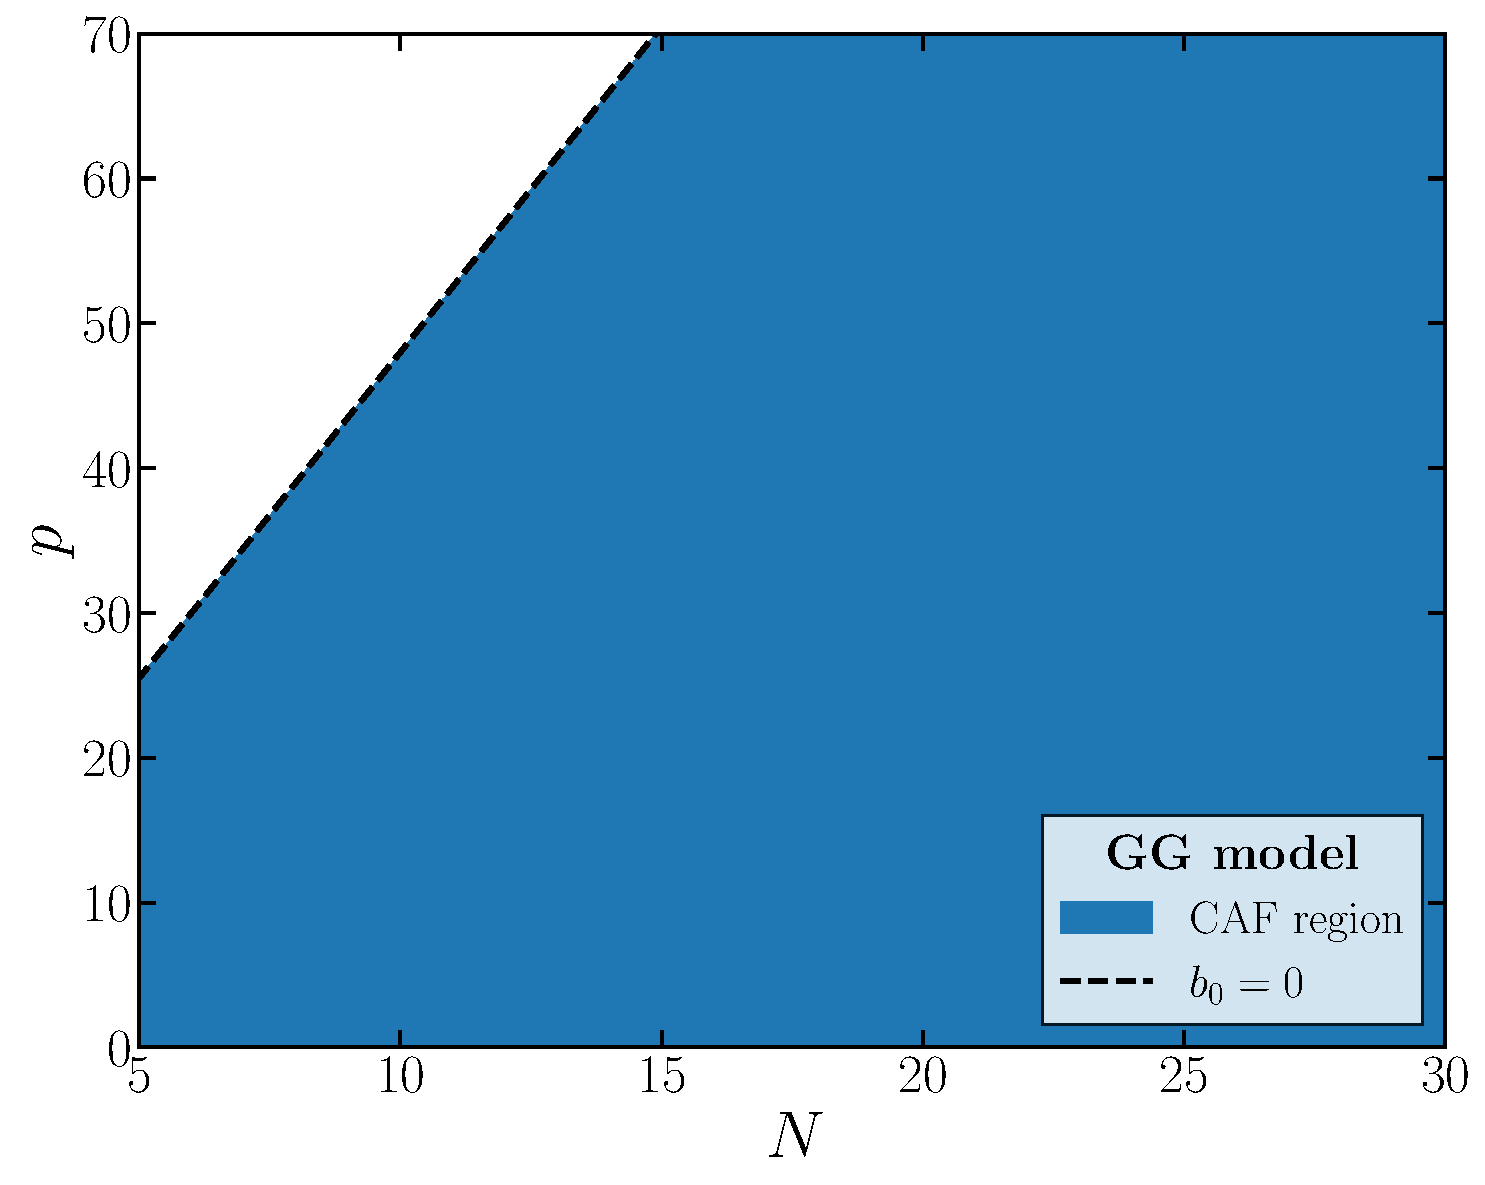
\includegraphics[width=\textwidth]{Figures/CAFGG_noscalar.pdf}
       \caption{GG model}
       \label{fig:noscalarGG}
   \end{subfigure}
   \hspace{0.1cm}
   \begin{subfigure}[b]{0.49\textwidth}
       \centering
       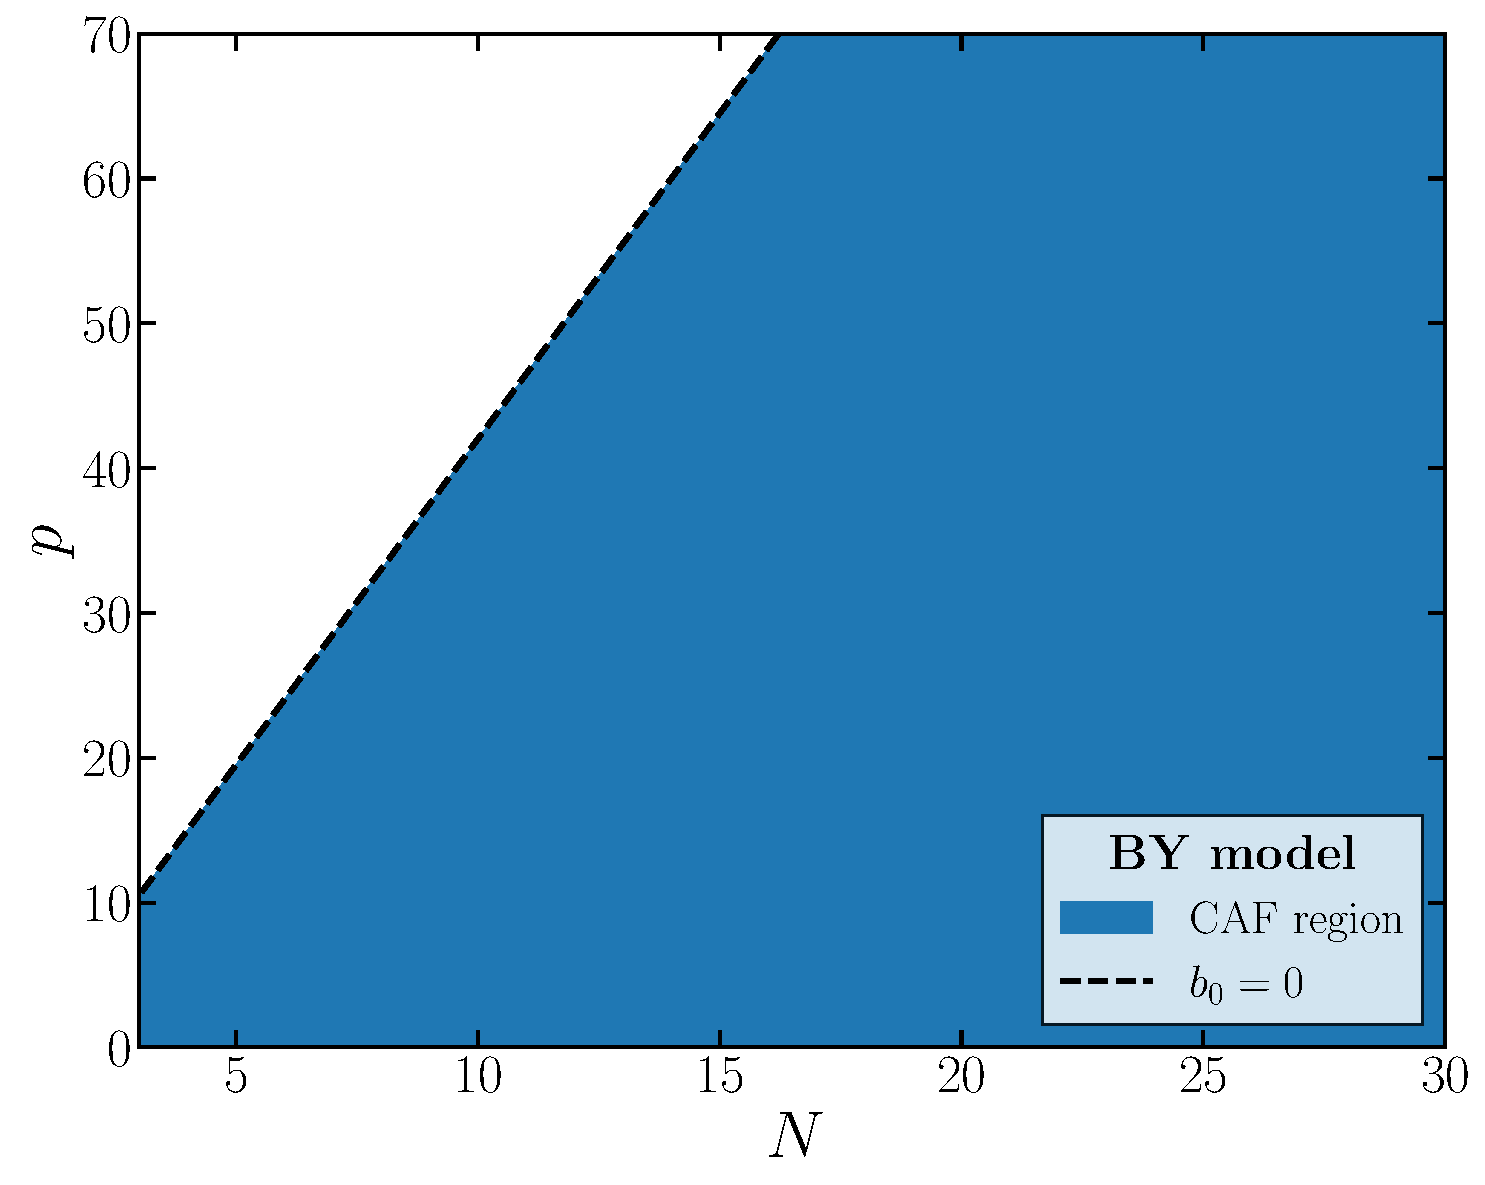
\includegraphics[width=\textwidth]{Figures/CAFBY_noscalar.pdf}
       \caption{BY model}
       \label{fig:noscalarBY}
   \end{subfigure}
   \caption{The figure illustrates the CAF region in parameter space ($N,p$) for (a) the GG model and (b) the BY model, without any scalars. The shaded blue area represents the CAF region, bounded by the dashed black line corresponding to the condition $b_0=0$. This boundary is given by the $p_{\max}$ function  Eq.~\eqref{eq:pNnoscalarGG} for the GG model and Eq.~\eqref{eq:pNnoscalarBY} for the BY model.}
   \label{fig:noscalar}
\end{figure} 
The gauge coupling thus creates an upper limit for the CAF region of the model and the GG model without scalars can therefore be CAF for all $N$, as seen in Figure~\ref{fig:noscalarGG}. 

\subsection{Scalar-Free Bars--Yankielowicz model}
We now focus on the BY model \cite{Bars:1981se}. Like the GG model, the BY model is a chiral model, the difference from the GG model is that the chiral fermion is in the two-index symmetric representation, i.e.\ $\chi_{ij}=\chi_{ji}$. This affects the anomaly coefficient of the field $A(\ytableausetup{boxsize=0.25cm}\begin{ytableau}{}&{}\end{ytableau})=(N+4)$. Effectively changing the copies of the anti-fundamental vector-like fermion to $q=N+4+p$, which ensures anomaly cancellation. This also changes the Dynkin index $T(\ytableausetup{boxsize=0.25cm}\begin{ytableau}{}&{}\end{ytableau})=\frac{N+4}{2}$, effectively changing the computation of the charges and will introduce a sign change to the $\U_1(1)$ charges, as seen in Table~\ref{tab:BY}.

Similar to the GG model, the BY model also has a lower boundary of the number of colours of the gauge group. The dimension of the two-index symmetric representation is $\frac{N(N+1)}{2}$. For $N=2$ this yields a dimension of $3$, which is the adjoint representation of the group, and thus is real \cite{Georgi:1999wka}, allowing for a Majorana mass term in the Lagrangian. For $\SU(3)$ the dimension is $6$ which is a complex representation. Resulting in a lower boundary of number of colours for the BY model: $N\ge3$. 

Thus, the Lagrangian is similar to that of the GG model and can be expressed as
\begin{align}\mathcal{L}= -\frac{1}{4} F_{\mu\nu}^a F^{a\mu\nu}+ i \bar{\chi}^{ij} \slashed{D} \chi_{ij} 
    + i \bar{\psi}^i_\alpha \slashed{D} \psi_i^\alpha 
    + i \bar{\tilde{\psi}}_i^\beta \slashed{D} \tilde{\psi}^i_\beta
    \,,
\end{align}
with similar index definitions as in Eq.~\eqref{eq:lGGnoscalar} except for the flavour index of the anti-fundamental fermion now given by $\beta=1,\dots, N+4+p$.

The gauge beta function can be found similarly to the GG model. The computation only differs in the number of anti-fundamental fermions: $N+4+p$, and the Dynkin index of the chiral fermion, yielding
\begin{align}
\sum T(R_f) &= \frac{N+2}{2} + \frac{N+4+p}{2} + \frac{p}{2} = N + 3 + p\,.
\end{align}
\begin{table}[b]
    \centering
    \renewcommand{\arraystretch}{1.5} 
    \begin{tabular}{|c|c|c|c|c|c|}
    \hline
    Fields & $\mathrm{SU}(N)$ & $\mathrm{SU}(N + 4 + p)$ & $\mathrm{SU}(p)$ & $\mathrm{U}_1(1)$ & $\mathrm{U}_2(1)$ \\
    \hline
    $\chi$ & $\ytableausetup{boxsize=0.25cm}\begin{ytableau}{}&{}\end{ytableau}$ & $1$ & $1$ & $N + 4$ & $2p$ \\

    $\tilde\psi$ & $\overline{\begin{ytableau}{}\end{ytableau}\rule{0pt}{7.5pt}}$ & $\overline{\begin{ytableau}{}\end{ytableau}\rule{0pt}{7.5pt}}$ & $1$ & $-(N + 2)$ & $-p$ \\

    $\psi$ & ${\begin{ytableau}{}\end{ytableau}}$ & $1$ & ${\begin{ytableau}{}\end{ytableau}}$ & $N +2$ & $-(N - p)$ \\
    \hline
    \end{tabular}
    \caption{Field content of the BY model. The table shows how the fields transform under the gauge and global symmetry groups, and their charges under the $\mathrm{U}_1(1)$ and $\mathrm{U}_2(1)$ symmetries.}
    \label{tab:BY} 
\end{table}
Thus, we obtain
\begin{equation}
    b_0=-\frac{2}{3}\left({9}N-6-2p\right) \,. \label{eq:betagaugeBY}
\end{equation}
This is similar the $b_0$ coefficient of the GG model in Eq.~\eqref{eq:betagauge}, up to the sign of the second term. Therefore the CAF region for the BY model is similar to that of the GG model. The conditions on the gauge beta function creates a comparable upper boundary which is given by
\begin{equation}
    p_{\text{max}}(N)=\frac{9N-6}{2} \,.\label{eq:pNnoscalarBY}
\end{equation} 
Thus, a CAF region exist for any N, as can be seen in Figure~\ref{fig:noscalarBY}.

Having now seen the two considered chiral models: the GG and the BY, it is time to introduce scalars into the mix. 
